% Created 2015-06-16 Tue 11:55
\documentclass[a4paper, titlepage]{tufte-handout}
        \usepackage[utf8]{inputenc}
\usepackage[T1]{fontenc}
\usepackage{textcomp}
\usepackage{footnote}
\usepackage{minitoc}
\usepackage{booktabs}
\usepackage{longtable}
\usepackage{lmodern}
\usepackage{graphicx}
\usepackage{url}
\usepackage{fancyvrb}
\usepackage{color}
\usepackage{xcolor}
\usepackage{amsmath}
\usepackage{amssymb}
\usepackage{mathabx}
\usepackage{mnsymbol}
\usepackage{array}
\usepackage{listings}
\usepackage{rotating}
\usepackage{multicol}
\usepackage{pdflscape}
\usepackage{ctable}
\usepackage{parskip}
\usepackage{anysize}
\usepackage{supertabular}
\usepackage{minted}
\usepackage{nicefrac}
\usepackage{units}
\usepackage{marginfix}
\usepackage{breakurl}
\usepackage{float}
\usepackage{placeins}
\usepackage{tabu}
\usepackage{tabulary}
\usepackage{tocloft}
\usepackage{titlesec}
\usepackage{titletoc}
\usepackage{changepage}
\usepackage{fancyhdr}
\usepackage{bibentry}
\usepackage{optparams}
\usepackage{paralist}
\usepackage{placeins}
\usepackage{ragged2e}
\usepackage{setspace}
\usepackage{textcase}
\usepackage{textcomp}
\usepackage{xifthen}
\usepackage{hyperref}
\usepackage{geometry}
\newcommand{\sectionbreak}{\clearpage}
\makeatletter
\renewcommand{\@tufte@reset@par}{\setlength{\RaggedRightParindent}{0pt}\setlength{\JustifyingParindent}{0pt}\setlength{\parindent}{0pt}\setlength{\parskip}{0.5\baselineskip}}
\@tufte@reset@par
\renewcommand{\@tufte@margin@par}{\setlength{\RaggedRightParindent}{0pt}\setlength{\JustifyingParindent}{0pt}\setlength{\parindent}{0pt}\setlength{\parskip}{0.5\baselineskip}}
\makeatother
\geometry{left=20mm, textwidth=130mm, marginparsep=8mm, marginparwidth=40mm}
\definecolor{darkblue}{rgb}{0,0,.5}
\definecolor{darkgreen}{rgb}{0,.5,0}
\definecolor{islamicgreen}{rgb}{0.0, 0.56, 0.0}
\definecolor{darkred}{rgb}{0.5,0,0}
\definecolor{mintedbg}{rgb}{0.95,0.95,0.95}
\definecolor{arsenic}{rgb}{0.23, 0.27, 0.29}
\definecolor{prussianblue}{rgb}{0.0, 0.19, 0.33}
\definecolor{coolblack}{rgb}{0.0, 0.18, 0.39}
\definecolor{cobalt}{rgb}{0.0, 0.28, 0.67}
\definecolor{moonstoneblue}{rgb}{0.45, 0.66, 0.76}
\definecolor{aliceblue}{rgb}{0.94, 0.97, 1.0}
\hypersetup{colorlinks=true, breaklinks=true, linkcolor=coolblack, anchorcolor=blue, citecolor=islamicgreen, filecolor=blue,  menucolor=blue,  urlcolor=violet, bookmarks=true, bookmarksopen=false, bookmarksdepth=3, bookmarksopenlevel=1, pagebackref=true, bookmarksnumbered=false, pdfstartview={Fit}, pdfpagelayout={SinglePage}}
\renewcommand\thefootnote{\textcolor{darkred}{\arabic{footnote}}}
\renewcommand{\theFancyVerbLine}{\sffamily\textcolor[rgb]{0.7,0.7,0.7}{\tiny\arabic{FancyVerbLine}}}
\setcounter{secnumdepth}{1}
\titleformat*{\section}{\LARGE\rmfamily\mdseries\itshape}
\renewcommand{\thesubsection}{\hspace*{-1.0em}}
\titlecontents{section} [0em] {\vspace{1\baselineskip}\Large\rmfamily\itshape}    {\hspace*{0em}} {\hspace*{0em}} {\rmfamily\itshape\qquad\thecontentspage} []
\renewcommand{\contentsname}{\LARGE\rmfamily\mdseries\itshape Contents\vspace{4\baselineskip}}
\setcounter{secnumdepth}{2}
\author{BNI, HPI, HZI, NFELTP, RKI, SAP}
\date{June 2015}
\title{SORMAS-N \protect\\ Tasks \& Logbook \protect\\ \LARGE Instructions for the Pilot Phase}
\hypersetup{
  pdfkeywords={},
  pdfsubject={},
  pdfcreator={Emacs 24.5.1 (Org mode 8.2.10)}}
\begin{document}

\maketitle
\renewcommand\plaintitle{SORMAS-N -- Tasks \& Logbook}
%\title{SORMAS-N Field Test -- Tasks \& Logbook}
%\author[The SORMAS Team]{BNI, HPI, HZI, NFELTP, RKI, SAP}
%\publisher{Publisher of This Book}

% Prints the month name (e.g., January) and the year (e.g., 2008)
\newcommand{\monthyear}{%
  \ifcase\month\or January\or February\or March\or April\or May\or June\or
  July\or August\or September\or October\or November\or
  December\fi\space\number\year
}

% .3 full title page
% \maketitle

% .4 copyright page
\newpage
% \begin{fullwidth}
~\vfill
\thispagestyle{empty}
%\setlength{\parindent}{0pt}
%\setlength{\parskip}{\baselineskip}

Copyright \copyright\ \the\year\ \thanklessauthor

% \par\smallcaps{Published by \thanklesspublisher}
% \par\smallcaps{sormas.googlecode.com}

\par 
Licensed under the Apache License, Version 2.0 (the ``License''); you may not
use this file except in compliance with the License. You may obtain a copy
of the License at \url{http://www.apache.org/licenses/LICENSE-2.0}. Unless
required by applicable law or agreed to in writing, software distributed
under the License is distributed on an \smallcaps{``AS IS'' BASIS, WITHOUT
WARRANTIES OR CONDITIONS OF ANY KIND}, either express or implied. See the
License for the specific language governing permissions and limitations
under the License.\index{license}

\par
\textit{First printing, \monthyear}
%\end{fullwidth}

% r.5 contents
\newpage
% \tableofcontents

\setcounter{tocdepth}{1}
\tableofcontents
\section{Introduction}
\label{sec-1}

This document contains some general remarks concerning the SORMAS-N field test and the daily tasks for all SORMAS roles.
Furthermore you can keep track of your work and experiences in a structured logbook every day. The booklet is concluded by a final assessment.
\subsection{Purpose of the System}
\label{sec-1-1}

SORMAS-N\footnote{Surveillance \& Outbreak Response Management System - Nigeria} was developed for two purposes. First, to assist public health workers in \emph{containing outbreaks of epidemic prone diseases}, where main aspects in containing the epidemic are contact tracing and outbreak management.
Second, to assist in \emph{systematically collecting routine data} on mandatory notifiable diseases as timely and exhaustive as possible.

\subsection{Purpose of the Pilot Phase}
\label{sec-1-2}

A 6-week pilot phase will test the \emph{usability} of SORMAS-N for those two purposes. During this phase, SORMAS-N will be tested in two Nigerian states, Oyo and Kano. In these states, smart-phones containing the SORMAS-N app will be distributed in the participating local government areas (LGAs) and the SORMAS-N desktop applications will be used at the respective state epidemiologist’s offices (see \hyperref[tab:roles]{Table 3}, \hyperref[tab:user-kano]{Table 4} and \hyperref[tab:user-oyo]{Table 5}). 

\begin{figure}[htb]
\centering
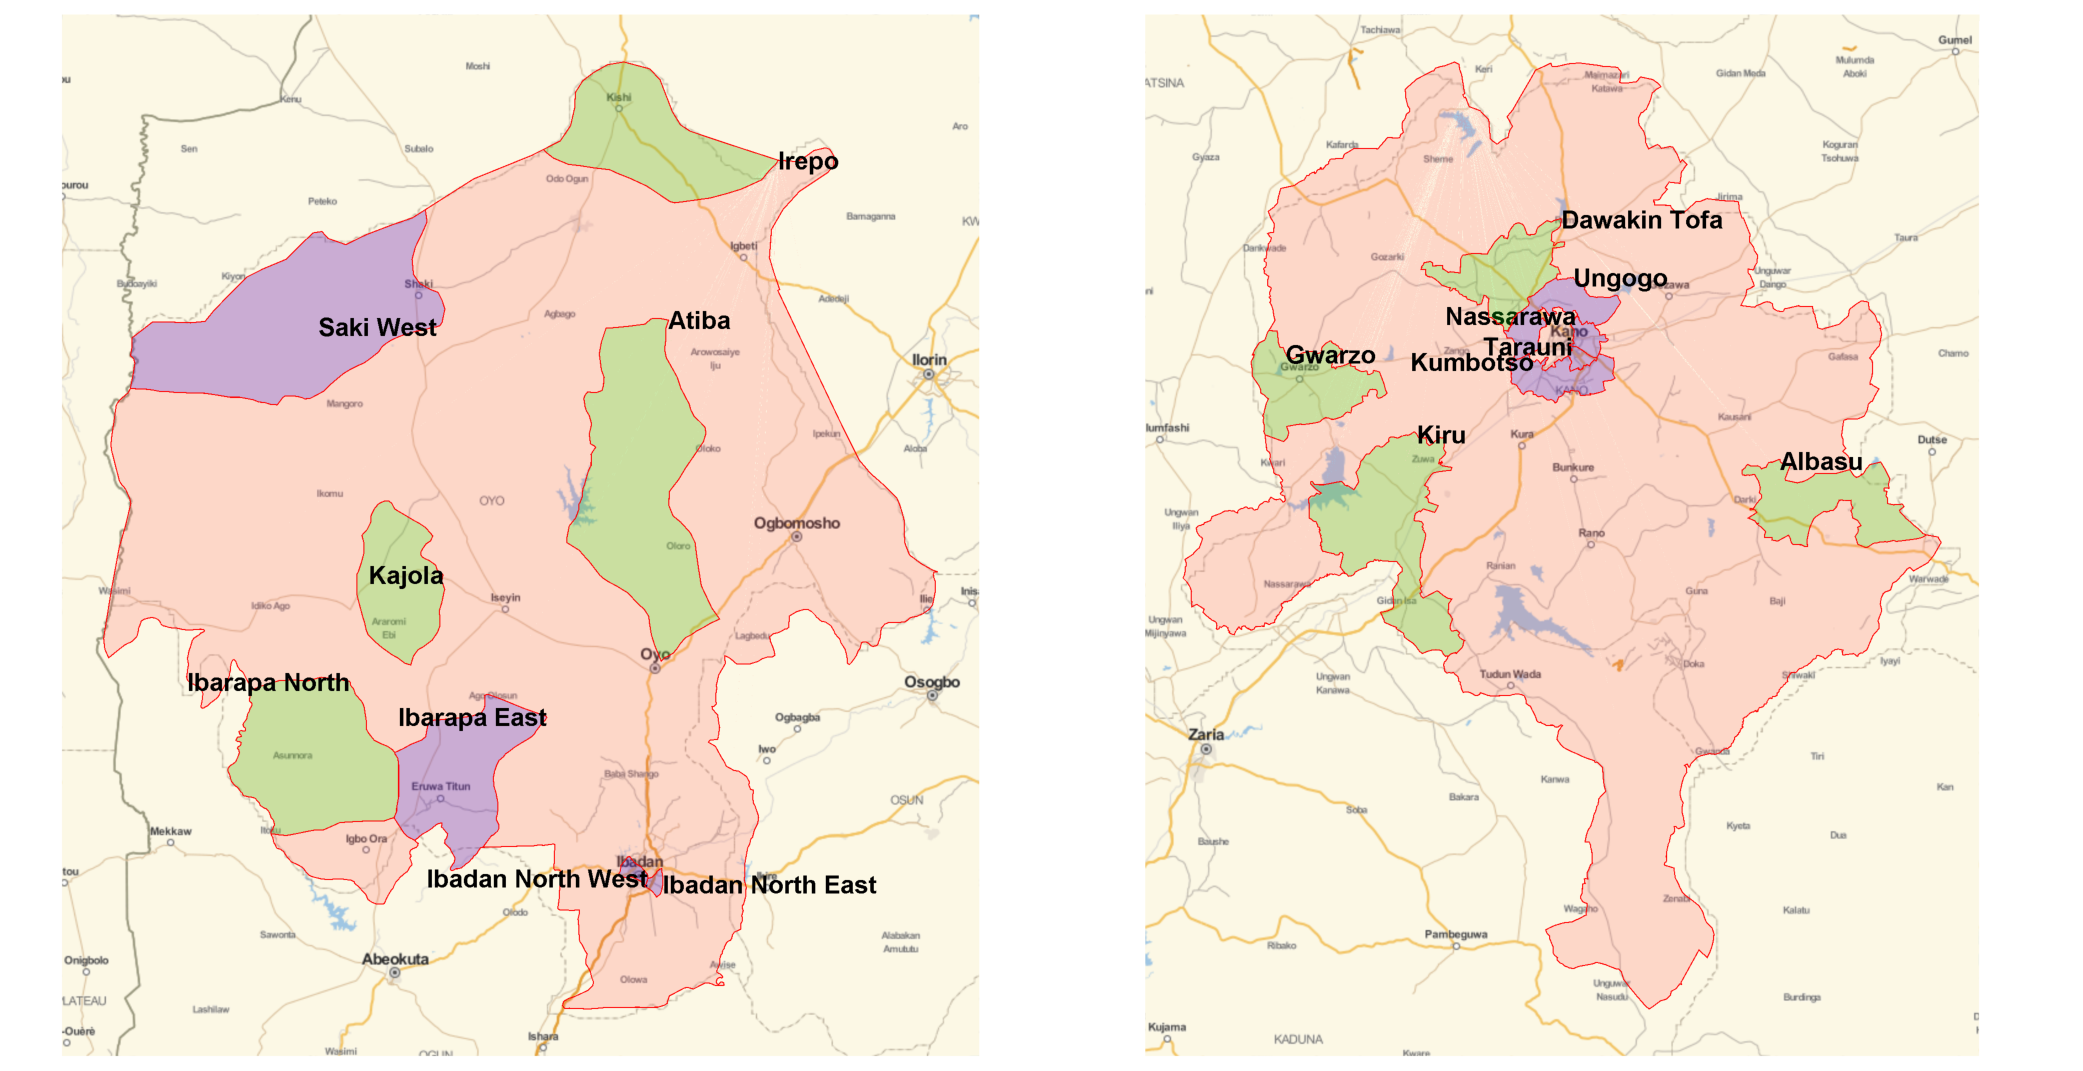
\includegraphics[height=180pt]{../../img/geo_lgas.pdf}
\caption{\label{fig:geo-lgas}The selected LGAs in Oyo and Kano.}
\end{figure}

\hyperref[tab:lgas]{Table 1} gives an overview of the LGAs participating in the field test.

\begin{table}[htb]
\caption{\label{tab:lgas}The selected LGAs with \emph{area type} and \emph{population}.}
\begin{tabular}{l|l|l|r|r}
\toprule
LGA & State & Area Type & Population & Area\\
\midrule
Albasu & Kano & rural & 190153 & 398\\
Dawakin Tofa & Kano & rural & 247875 & 479\\
Gwarzo & Kano & rural & 183987 & 393\\
Kiru & Kano & rural & 264781 & 927\\
Kumbotso & Kano & urban & 295979 & 158\\
Nassarawa & Kano & urban & 596669 & 34\\
Tarauni & Kano & urban & 221367 & 28\\
Ungogo & Kano & urban & 369657 & 204\\
Atiba & Oyo & rural & 169702 & 1757\\
Ibadan North East & Oyo & urban & 330399 & 18\\
Ibadan North West & Oyo & urban & 152834 & 26\\
Ibarapa East & Oyo & urban & 118226 & 838\\
Ibarapa North & Oyo & rural & 101092 & 1218\\
Irepo & Oyo & rural & 122553 & 984\\
Kajola & Oyo & rural & 200997 & 609\\
Saki West & Oyo & urban & 278002 & 2014\\
\bottomrule
\end{tabular}
\end{table}
\medskip


During the pilot phase, every person participating in the SORMAS-N test will be required to carry out certain tasks and enter data daily via the smart-phone or the desktop application during the days of Monday to Friday.

As SORMAS was developed for two different purposes, these are tested in 2 different ways:

\begin{enumerate}
\item \emph{Exercise disease} -- to see how SORMAS assists in contact tracing and management of an outbreak prone disease (e.g. Ebola), participants will be provided with daily information on a mock-disease called exercise disease\footnote{ExD -- \emph{exercise disease}}, blurred by cases of a clinically similar disease called other febrile disease\footnote{OFD -- \emph{other febrile disease}}, that can reliably be distinguished from exercise disease by lab diagnosis only. This data comes from a simulated scenario and all data will be generated by a computer. It will give an impression of an outbreak with cases and contact persons as realistic as possible – but names, places and stories are invented. This invented data is to be entered according to the role (see below) each participant takes on.

\item \emph{Routine data collection} -- three different diseases\footnote{3D -- \emph{Measles, Cholera and Avian Influenza}} were chosen to test SORMAS’ usefulness in collecting routine data: Measles, Cholera and Avian Influenza\footnote{AI -- \emph{Avian Influenza}}. 
This data needs to be entered daily in SORMAS-N in addition to the paper based forms that are already in use and currently collected weekly. These are real data and depend on their appearance in the respective LGAs. They are not coming from a simulation. Therefore, every case of those 3 diseases seen in the LGAs should appear twofold: on a paper form and in SORMAS-N. The data on paper will be collected in the usual way by the DSNO. 

For \emph{Hospital focal persons} and \emph{Surveillance officers} a difference to the current practice will be, that you will also be required to enter information daily even if there are no cases of measles, cholera and avian flu (daily zero-reporting).
\end{enumerate}

\subsection{User Roles}
\label{sec-1-3}

As demonstrated in the training, during an outbreak of an epidemic prone disease, there would be an organizational framework called \emph{Emergency Operation Center (EOC)} to manage the different surveillance and outbreak information and activities. Within this framework, people take on different roles with different preset tasks, depending on their background. This is reflected in SORMAS. Every user of SORMAS has its unique role. All roles are briefly sketched. In the following sections your role and tasks are outlined in more detail.

A \emph{Hospital focal person} (aka \emph{Informant}) collects information on illness and death among patients and health care workers in a health facility and enters this information into SORMAS-N.

A \emph{Surveillance officer} collects information on \emph{exercise disease} and the 3 selected mandatory notifiable diseases in the community. She verifies and completes information on rumors according to her investigation. She assures daily notification of all suspected and confirmed cases of Measles, Cholera, Avian Influenza occurring in the LGA. This includes daily zero-notification of these 3 diseases, if no cases have occurred.

The \emph{Rumor officer} triages and processes incoming rumors on \emph{exercise disease} and forwards them to the \emph{Surveillance supervisor}.

The \emph{Surveillance supervisor} manages and coordinates information received from the \emph{Rumor officer} and the \emph{Surveillance officers}. She decides on investigating a new rumor. 

A \emph{Contact officer} is responsible for all aspects of contact tracing of contact persons. For Avian Influenza, this concerns human and animal cases. For \emph{exercise disease} this includes daily visits of contact persons, assessing and documenting symptoms and notifying new possible cases.

The \emph{Contact supervisor} is responsible for coordination of the contact management of \emph{exercise disease} and Avian Influenza. She is responsible for all \emph{Contact officers} within her state. She informs the \emph{Case supervisor} about symptomatic contact persons and hands over suspected cases for further management, e.g. evacuation, isolation, lab confirmation, decontamination or psycho-social support.

The \emph{Case supervisor} coordinates all activities around the case management (i.e. clinical management, isolation measures, transport, decontamination of residences or facilities, burial, psycho-social support). She immediately communicates results of laboratory investigations in case of \emph{exercise disease} and Avian Influenza and thereby updates the status of \emph{suspected cases} to \emph{confirmed cases}, \emph{probable cases}, \emph{non-cases} or \emph{discarded cases} resp..


\hyperref[tab:roles]{Table 2} gives an overview of the distribution of the participants and their roles. 

\begin{table*}[htb]
\caption[The distribution of roles][0\baselineskip]{The distribution of participants according to their role, facility type and state.}\label{tab:roles}
\begin{tabular}{ll|rr|r}
\toprule
SormasRole & FacilityType & Kano & Oyo & (all)\\
\midrule
Case supervisor & Tertiary & 1 & 0 & 1\\
Case supervisor & NA & 0 & 1 & 1\\
Contact officer & NA & 8 & 8 & 16\\
Hospital focal person & Primary & 28 & 9 & 37\\
Hospital focal person & Secondary & 4 & 14 & 18\\
Hospital focal person & Tertiary & 1 & 2 & 3\\
Hospital focal person & NA & 0 & 8 & 8\\
Rumor officer & NA & 1 & 1 & 2\\
Surveillance \& Contact supervisor & NA & 1 & 1 & 2\\
Surveillance officer & NA & 8 & 8 & 16\\
(all) & (all) & 52 & 52 & 104\\
\bottomrule
\end{tabular}
\end{table*}

\medskip

\subsection{Data for Exercise Disease}
\label{sec-1-4}

This booklet gives you an overview of the daily tasks on \emph{exercise disease} for each role. In a supplementing document individual information including all injects will be given to each participant. It will contain data that should be entered by you which have been generated by the SORMAS simulation, and are invented especially for this pilot. These guided tasks will trigger further action resulting in additional data. All these \emph{resulting data} will then be compared with the \emph{expected data} to provide another evaluation method. On selected weekends during the pilot phase it is planed to adjust the data to the simulated story line. 

\emph{Entries by the users are made from Monday to Friday only. Entries by the system will be made on weekends only.}


\subsection{The Logbook}
\label{sec-1-5}

This booklet contains for each day of the pilot phase a page -- the log -- which is left for users’ comments and feedback. It is meant to document any problems or experiences that may occur. It is very important to document any difficulties or problems that occurred – this will help us to improve SORMAS.


\subsection{Help!}
\label{sec-1-6}

If you feel that the SORMAS-N manual is not sufficient to answer your questions, the \emph{SORMAS-N helpline} is available, where the following persons (see \hyperref[tab:help]{Table 3}) can assist you.

\begin{table}[htb]
\caption{\label{tab:help}The SORMAS-N helpline.}
\begin{tabular}{l|l|l}
\toprule
Mr. Gbolagade Rasaki & 0706-5523575 & \href{mailto:g.rasaki@sormas.ng}{g.rasaki@sormas.ng}\\
Dr. Ebiwumi Aikhionbare & 038-6174455 & \href{mailto:e.aikhionbare@sormas-n.org}{e.aikhionbare@sormas-n.org}\\
Mr. Adebowale Olofinmoyin & +234-801-6076028 & \href{mailto:a.olofinmoyin@sormas.net}{a.olofinmoyin@sormas.net}\\
\bottomrule
\end{tabular}
\end{table}

\subsection{List of Participants}
\label{sec-1-7}

\hyperref[tab:user-kano]{Table 4} and \hyperref[tab:user-oyo]{Table 5} list all participants from Kano and Oyo participating in the field test.

\begin{table*}\footnotesize
\caption[The participants of Kano.][1.2\baselineskip]{The participants of Kano.}\label{tab:user-kano}
\begin{tabular}{l|l|l|l}
\toprule
LGA & SormasRole & Institution & Name\\
\midrule
Albasu & Contact officer & LGA HD & Mr Nonso Fabunmi\\
Albasu & Hospital focal person & Albasu PHC & Mr Sesugh Ogunode\\
Albasu & Hospital focal person & Fanda PHC & Mr Ugoh Maduabum\\
Albasu & Hospital focal person & Hungu PHC & Mrs Chiburem Dabiri\\
Albasu & Hospital focal person & Tsangaya PHC & Mr Azi Aikhionbare\\
Albasu & Surveillance officer & LGA HD & Mr Adebolajo Oboli\\
Dawakin Tofa & Contact officer & LGA HD & Mr Nnaemeka Mbah\\
Dawakin Tofa & Hospital focal person & Dandalama PHC & Mr Godwin Fajinmi\\
Dawakin Tofa & Hospital focal person & Dawanau PHC & Mrs Mujee Bot Kan\\
Dawakin Tofa & Hospital focal person & Tattarawa PHC & Mrs Loutoyopnica Kanayo\\
Dawakin Tofa & Hospital focal person & Dawaki General hospital & Mrs Al Derafaka Aradeon\\
Dawakin Tofa & Surveillance officer & LGA HD & Mrs Njideka Emordi\\
Gwarzo & Contact officer & LGA HD & Mrs Ijeoma Ezinwa\\
Gwarzo & Hospital focal person & Getso MCH & Mr Yakubu Effiom\\
Gwarzo & Hospital focal person & Alheri Clinic & Mr Adeyemi Njoku\\
Gwarzo & Hospital focal person & Koya Health Post & Mr Enosaze Olowola\\
Gwarzo & Hospital focal person & Gwarzo General Hospital & Mr Uche Mohamed\\
Gwarzo & Surveillance officer & LGA HD & Mr Olaoluwa Mshelia\\
Kiru & Contact officer & LGA HD & Mr Akinola Ohen\\
Kiru & Hospital focal person & Kiru CHC & Mrs Ololade Ogunbanwo Sosan\\
Kiru & Hospital focal person & Yako BCH & Mrs Tamunodieprieye Emigo\\
Kiru & Hospital focal person & Stholic Clinic & Mr Okoro Keita\\
Kiru & Hospital focal person & Taimako Clinic & Mr Omolade Bird\\
Kiru & Surveillance officer & LGA HD & Mr Oladipo Giwa\\
Kumbotso & Contact officer & LGA HD & Mrs Oluwanifesimi Abayomi\\
Kumbotso & Hospital focal person & Chiranci PHC & Mrs Adeyinka Olowola\\
Kumbotso & Hospital focal person & Sheka PHC & Mr Onyinye Agwuocha\\
Kumbotso & Hospital focal person & Nasiha Clinic & Mr Osagie Bada\\
Kumbotso & Hospital focal person & Tajudden Clinic & Mr Mosaku Choji\\
Kumbotso & Surveillance officer & LGA HD & Mrs Olamide Popoola\\
Nassarawa & Contact officer & LGA HD & Mrs Stella Uzochukwu\\
Nassarawa & Hospital focal person & Gwagwarwa PHC & Mrs Gberbo Ikeke\\
Nassarawa & Hospital focal person & Ahmadiyya Hospital & Mr Chinzor Oyeledun\\
Nassarawa & Hospital focal person & Bamaiyi Hospital & Mrs Ciara Emedolu\\
Nassarawa & Hospital focal person & Sir Muhd Sunusi Hospital & Mr Oladipo Ikimi\\
Nassarawa & Surveillance officer & LGA HD & Mr Chidi Sherif\\
Tarauni & Contact officer & LGA HD & Mrs Omodolapo Atulewa\\
Tarauni & Hospital focal person & Ja'oji PHC & Mr Ibinabo Ararume\\
Tarauni & Hospital focal person & Unguwa Uku PHC & Mrs Oluwaseyanu Adadevoh\\
Tarauni & Hospital focal person & Almu Hospital & Mr Ogbu Iyam\\
Tarauni & Hospital focal person & Annoury Hospital & Mrs Isobel Henry Akarandut\\
Tarauni & Surveillance officer & LGA HD & Mr Osagie Effiom\\
Ungogo & Contact officer & LGA HD & Mrs Fanique Inoniyegha\\
Ungogo & Hospital focal person & Ungogo PHC & Mr Ovieoghene Kanayo\\
Ungogo & Hospital focal person & Rahama Clinic & Mr Affiong Nworuh\\
Ungogo & Hospital focal person & Unicare Hospital & Mrs Olasubomi Olomu\\
Ungogo & Hospital focal person & Waziri Shehu Gidado & Mrs Chiapali Iyorhe\\
Ungogo & Surveillance officer & LGA HD & Mr Oseremen Ojukwu\\
NA & Case supervisor & Yar Gaya Hospital & Mr Ighogbetine Nguirmamaramama\\
NA & Hospital focal person & Yar Gaya Hospital & Mr Ogadinma Kontagora\\
NA & Rumor officer & State HD & Mrs Tarela Idahor\\
NA & Surveillance \& Contact supervisor & State HD & Mr Adebowale Agbebaku\\
\bottomrule
\end{tabular}
\end{table*}

\begin{table*}\footnotesize
\caption[The participants of Oyo.][1.2\baselineskip]{The participants of Oyo.}\label{tab:user-oyo}
\begin{tabular}{l|l|l|l}
\toprule
LGA & SormasRole & Institution & Name\\
\midrule
Atiba & Contact officer & LGA HD & Mrs Chisom Ihenacho\\
Atiba & Hospital focal person & Grace Hospital & Mrs Oni Ezeife\\
Atiba & Hospital focal person & Oroki Medical Centre & Mr Arome Ubido\\
Atiba & Hospital focal person & Boroboro Health centre & Mrs Chizoba Sodje\\
Atiba & Hospital focal person & State Hospital & Mr Adedeji Obanor\\
Atiba & Surveillance officer & LGA HD & Mr Ok Kefee\\
Ibadan North East & Contact officer & LGA HD & Mr Nonso Oguntokun\\
Ibadan North East & Hospital focal person & Jobi Memorial Hospital, Paadi & Mrs Ibukunoluwa Ebor\\
Ibadan North East & Hospital focal person & Iwo road Health Centre & Mr Akindela Maduabum\\
Ibadan North East & Hospital focal person & OkeAdu Health Centre & Mrs Oluremi Bali\\
Ibadan North East & Hospital focal person & Oluyoro Catholic Hospital & Mr Osabuhien Ofere\\
Ibadan North East & Surveillance officer & LGA HD & Mrs Plangnan Idahor\\
Ibadan North West & Contact officer & LGA HD & Mr Godwin  Eguavoen\\
Ibadan North West & Hospital focal person & Ayeye Primary Health Centre & Mrs Onayi Nwuche\\
Ibadan North West & Hospital focal person & Jericho Specialist Hospital & Mrs Adaobi Chiejine\\
Ibadan North West & Hospital focal person & AlafiaHospital & Mr Akinola Rasaki\\
Ibadan North West & Hospital focal person & Unity Medical Centre & Mrs Nadoca Guda\\
Ibadan North West & Surveillance officer & LGA HD & Mrs Toniah Egerega\\
Ibarapa East & Contact officer & LGA HD & Mrs Omodolapo Uduak\\
Ibarapa East & Hospital focal person & Oke Imale primary health centre & Mr Kingsley  Onyemachi\\
Ibarapa East & Hospital focal person & General Hospital, Eruwa & Mr Aryee Ezenwaka\\
Ibarapa East & Hospital focal person & Awojobi Clinic & Mrs Adaeze Keita\\
Ibarapa East & Hospital focal person & Rehoboth Hospital & Mrs Mesoma Ubah\\
Ibarapa East & Surveillance officer & LGA HD & Mrs Anike Ibe\\
Ibarapa North & Contact officer & LGA HD & Mr Ogadinma Elumelu\\
Ibarapa North & Hospital focal person & Akindele Clinic & Mr Ime  Iyke\\
Ibarapa North & Hospital focal person & Victory foundation & Mr Oludare Omodiagbe\\
Ibarapa North & Hospital focal person & PHC Okeola & Mr Edoja Oshoala\\
Ibarapa North & Hospital focal person & General Hospital & Mr Olatunbosun Ekoku\\
Ibarapa North & Surveillance officer & LGA HD & Mr Decale Oya Decale Aminu\\
Irepo & Contact officer & LGA HD & Mr Madukairo Katsina\\
Irepo & Hospital focal person & Elkeedam Clinic & Mrs Oula Omeje\\
Irepo & Hospital focal person & Agede PHC & Mrs Stella Ogungbe\\
Irepo & Hospital focal person & Kisi General Hospital & Mr Olatunbosun Azeez\\
Irepo & Hospital focal person & Muslim Hospital & Mrs Adaobi Mshelia\\
Irepo & Surveillance officer & LGA HD & Mrs Odera Envoh\\
Kajola & Contact officer & LGA HD & Mr Chimere Oboh\\
Kajola & Hospital focal person & Baptist Medical centre Okeho & Mr Okoro Osuchukwu\\
Kajola & Hospital focal person & Wuraola Hospital & Mr Niamke Isa\\
Kajola & Hospital focal person & Ijo Primary Health Care Centre & Mr Olatunbosun Kontagora\\
Kajola & Hospital focal person & Okeho General Hospital & Mrs Temilore Brann\\
Kajola & Surveillance officer & LGA HD & Mr Clinton Iyke\\
Saki West & Contact officer & LGA HD & Mrs Oluwafunke Agbamuche\\
Saki West & Hospital focal person & Isale Taba Maternity Centre & Mr Oluwakemi Kontagora\\
Saki West & Hospital focal person & State Hospital & Mrs Bukola Onyearugbulem\\
Saki West & Hospital focal person & Baptist Medical Centre & Mrs Efuose Omoko\\
Saki West & Hospital focal person & Muslim Hospital & Mr Ovieoghene Yaji\\
Saki West & Surveillance officer & LGA HD & Mrs Omotese Ogugua\\
NA & Case supervisor & Isolation unit & Mrs Ololade Vanzekin\\
NA & Hospital focal person & IDSR UCH & Mrs Mujeedat Dabiri\\
NA & Rumor officer & State HD & Mrs Omodolapo Okafor\\
NA & Surveillance \& Contact supervisor & State HD & Mr Irechukwu Akinfenwa\\
\bottomrule
\end{tabular}
\end{table*}

\newpage
\section{Hospital Focal Person (Informant)}
\label{sec-2}

\subsection{Tasks as Hospital Focal Person (3D)}
\label{sec-2-1}

Concerning Measles, Cholera and Avian Influenza\footnote{according to occurrence of real cases}:

\emph{\textcolor{gray}{daily}}

\begin{enumerate}
\item Notify any case of these 3 diseases via SORMAS-N as well as via established IDSR procedures (paper) to the \emph{Surveillance officer} of your LGA.

\item Send a daily zero-report of those 3 diseases via SORMAS-N (when applicable).
\end{enumerate}

\subsection{Tasks as Hospital Focal Person (ExD)}
\label{sec-2-2}

Concerning exercise disease\footnote{according to the daily information given in the tasks section of the day}:

\emph{\textcolor{gray}{before 10 AM}}

\begin{enumerate}
\item You have the following information about patients or health care workers in your facility about \emph{exercise disease}. Use them to fulfill your duty as a \emph{Hospital focal person}.

\emph{\ldots list of possible cases (person information with symptoms)}
\end{enumerate}


\begin{enumerate}
\item Some patients have died. Please notify this via SORMAS-N.

\emph{\ldots list of persons that have died}
\end{enumerate}

\section{Rumor Officer}
\label{sec-3}

\subsection{Tasks as Rumor Officer (3D)}
\label{sec-3-1}

\emph{Concerning Measles, Cholera and Avian Influenza you have no tasks.}

\subsection{Tasks as Rumor Officer (ExD)}
\label{sec-3-2}

Concerning exercise disease\footnote{according to the daily information given in the tasks section of the day}:

\emph{\textcolor{gray}{before 10 AM}}

\begin{enumerate}
\item Enter the following rumors.

\begin{itemize}
\item Enter rumor information.

\item Enter place information connected to the rumor.

\item Enter person information connected to the rumor.

\item Enter possible cases related to the rumor. Mark them as \emph{possible case}.

\item Enter contact person information.
\end{itemize}

\emph{\ldots daily list of rumors}

\emph{\ldots sometimes with participating persons and possibly with their symptoms}

\emph{\ldots each rumor ends with a $\blacksquare$}

\item You have received information about cases of death. Please notify them via SORMAS-N.

\emph{\ldots list of persons that have died}
\end{enumerate}

\section{Surveillance Officer}
\label{sec-4}

\subsection{Tasks as Surveillance Officer (3D)}
\label{sec-4-1}

Concerning Measles, Cholera and Avian Influenza\footnote{according to occurrence of real cases}:

\emph{\textcolor{gray}{daily}}

\begin{enumerate}
\item Notify any case of those 3 diseases via SORMAS-N as well as via established IDSR procedures (paper) to your \emph{Surveillance supervisor}. Every time there is such a case, please make a photocopy of each IDSR notification. Collect daily copies until the end of the pilot phase and hand them over together with the booklet to Dr. Olawunmi Adeoye.

\item Perform a daily zero-reporting if no cases occur.
\end{enumerate}

\subsection{Tasks as Surveillance Officer (ExD)}
\label{sec-4-2}

Concerning exercise disease\footnote{according to the daily information given in the tasks section of the day}:

\emph{\textcolor{gray}{before 10 AM}}

\begin{enumerate}
\item Verify and complete information on rumors according to your investigation on site, which have resulted in the following information.

\begin{itemize}
\item Complete rumor information.

\item Complete place information connected to the rumor.

\item Complete person information connected to the rumor.

\item Complete possible cases related to the rumor. Mark them as \emph{possible case}.
\end{itemize}

\emph{\ldots daily list of rumors}

\emph{\ldots sometimes with participating persons and possibly with their symptoms}

\emph{\ldots each rumor ends with a $\blacksquare$}

\item In your investigation you have identified the following new contacts (of persons which had contact to a known case). Enter them into SORMAS-N.

\emph{\ldots list of contacts (persons with case information)}
\end{enumerate}

\emph{\textcolor{gray}{after 3 PM}}

\begin{enumerate}
\setcounter{enumi}{2}
\item Look for new reports of \emph{possible cases}. Complete the missing information. 

\emph{\ldots list of cases (persons with symptoms)}

\item Look for new reports of cases of death. Confirm the information.

\emph{\ldots list of persons that have died}
\end{enumerate}

\section{Contact Officer}
\label{sec-5}

\subsection{Tasks as Contact Officer (AI)}
\label{sec-5-1}

\emph{Concerning Measles and Cholera you have no tasks.}

Concerning Avian Influenza\footnote{according to occurrence of real cases}:

\emph{\textcolor{gray}{daily}}

\begin{enumerate}
\item Notify contact persons of animal and human cases of Avian Influenza including zero-notifications.

\item Visit contact persons to check and document any symptoms of Avian influenza for 17 consecutive days.
\end{enumerate}


\subsection{Tasks as Contact Officer (ExD)}
\label{sec-5-2}

Concerning exercise disease\footnote{according to the daily information given in the tasks section of the day}:

\emph{\textcolor{gray}{between 11 AM and 2PM}}

\begin{enumerate}
\item Display the list of all your tasks.

\emph{\ldots number of task}

\item You are visiting contact persons. While you do your visits, you retrieve the following information.

\begin{itemize}
\item Is the person available and cooperative?

\item Enter the contact visit information.

\item Create an appointment for the next visit.
\end{itemize}
\emph{\ldots daily list of visit information}

\item Mark the following visits as \emph{not possible}.

\emph{\ldots daily list of schedule entries of visit which were not possible}

\item During your visit you learned about additional contact persons and contact information (contact person in contact with case). Enter them into SORMAS-N.

\emph{\ldots daily list of contact information}

\item During your visit you learned about cases of death. Enter this information into SORMAS-N.

\emph{\ldots list of persons that have died}
\end{enumerate}

\section{Surveillance and Contact Supervisor}
\label{sec-6}

\subsection{Tasks as Surveillance Supervisor (3D)}
\label{sec-6-1}

Concerning Measles, Cholera and Avian Influenza\footnotemark[11]{}:

\emph{\textcolor{gray}{daily}}

\begin{enumerate}
\item Check the list of notified cases including zero-notifications.

\item Check, validate and manage any other incoming information of the \emph{Surveillance officers}.

\item Create tasks when necessary and assign them to your \emph{Surveillance officers}.
\end{enumerate}

\subsection{Tasks as Contact Supervisor (AI)}
\label{sec-6-2}

\emph{Concerning Measles and Cholera you have no tasks.}

Concerning Avian Influenza\footnote{according to occurrence of real cases}:

\emph{\textcolor{gray}{daily}}

\begin{enumerate}
\item Create follow-up tasks (for 17 days, including first and final visit) for contact persons of a suspected or confirmed human or animal case of Avian Influenza.

\item Assign tasks to \emph{Contact officers}.

\item List all contact persons with symptoms.

\item Have a look at each case and confirm those who fulfill the case definition. Immediately trigger action as appropriate.
\end{enumerate}

\subsection{Tasks as Surveillance Supervisor (ExD)}
\label{sec-6-3}

\emph{\textcolor{gray}{between 11 AM and 2 PM}}

\begin{enumerate}
\item List all rumors (the new ones highlighted) with \emph{possible cases} and contact persons.
\item Have a look at each \emph{possible case} and confirm those who fulfill the case definition as \emph{suspected case}.
\end{enumerate}

\emph{\textcolor{gray}{after 3 PM}}

\begin{enumerate}
\setcounter{enumi}{2}
\item Create a surveillance report.

\item Look at the rumor list and decide on the status of each rumor. Create necessary tasks for further investigation and assign them to \emph{Surveillance officers}.
\end{enumerate}

\newpage
\subsection{Tasks as Contact Supervisor (ExD)}
\label{sec-6-4}

\emph{\textcolor{gray}{before 10 AM}}

\begin{enumerate}
\item Are any of the newly entered contact persons or contacts already in the system? Confirm all contact persons entered by the \emph{Contact officers}.

\item Create tasks for initial visits, contact visits and final visits for all new contact persons.

\item Assign all unassigned tasks to the \emph{Contact officer} of the LGA where the contact person resides.
\end{enumerate}

\emph{\textcolor{gray}{after 3 PM}}

\begin{enumerate}
\setcounter{enumi}{3}
\item List all contact persons with symptoms (\emph{possible cases}).

\item Have a look at each \emph{possible case} and confirm those who fulfill the case definition as \emph{suspected case}.

\item List all contact persons of cases with 2 negative lab results (\emph{non-cases}) that are still in contact tracing. Stop the contact tracing and create a final visit.

\item Check the status of the assigned tasks. Look for tasks that are overdue.
\end{enumerate}
 

\section{Case Supervisor}
\label{sec-7}

\subsection{Tasks as Case Supervisor (3D)}
\label{sec-7-1}

Concerning Measles, Cholera and Avian Influenza\footnote{according to occurrence of real cases}:

\emph{\textcolor{gray}{daily}}

\begin{enumerate}
\item Coordinate the \emph{Case officers} for clinical management of cases and case management.\footnote{\emph{Case officer} is currently not a user role of SORMAS.}
\end{enumerate}

\subsection{Tasks as Case Supervisor (ExD)}
\label{sec-7-2}

Concerning exercise disease\footnote{according to the daily information given in the tasks section of the day

\newpage}:

\emph{\textcolor{gray}{before 10 AM}}

\begin{enumerate}
\item Are there any cases that must be isolated? Display the list of all those cases. Create tasks for isolation for those cases who need it and assign it.

\item Are there any cases that need lab diagnosis? Display the list of all those cases. Create tasks for lab diagnostic verification for those cases who need it and assign it.

\item Display all lab requests that are overdue.

\emph{\ldots number of requests overdue}

\item You receive the following lab information. Make sure it is properly documented in SORMAS-N.

\emph{\ldots lab information for cases}

\item Are there any cases that can be discharged? Display the list of all those cases. Create tasks for those cases who need it and assign it.
From those that have two negative tests (48h apart) the following cases are symptom-free for at least 3 days. 

\emph{\ldots list of cases (name with birth date)}

\item Are there any cases who died? Display the list of all those cases. Create tasks for the burial of those cases who need it and assign it.

\emph{\ldots list of cases (name with birth date)}
\end{enumerate}

\emph{\textcolor{gray}{after 3 PM}}

\begin{enumerate}
\setcounter{enumi}{6}
\item Are there any tasks that need to be updated? Display a list of pending tasks and update their status.

\emph{\ldots list of tasks (name of case, task type and status)}
\end{enumerate}
\section{Logbook}
\label{sec-8}


\subsection{Day 1 -- 2015-06-01 -- Mon  1 Jun}
\label{sec-8-1}
\begin{enumerate}
\item How did you execute the \emph{exercise disease} tasks in SORMAS-N today?

\quad $\square$ without difficulties

\quad $\square$ with some difficulties

\quad $\square$ unable to fully execute the tasks

\quad $\square$ unable to execute the tasks

\quad $\square$ not applicable, as there were no tasks for \emph{exercise disease} today

\item How did you execute your task of notifying \emph{Measles, Cholera or Avian Influenza} cases in SORMAS-N today?

\quad $\square$ without difficulties

\quad $\square$ with some difficulties

\quad $\square$ unable to notify via SORMAS-N

\quad $\square$ not applicable, as there were no such cases today

\item Please give detailed description of the problem if you encountered any difficulties either with notification of \emph{Measles, Cholera or Avian Influenza} cases or with the execution of the exercise.

\hrulefill

\hrulefill

\hrulefill

\hrulefill

\hrulefill

\hrulefill

\hrulefill

\hrulefill

\hrulefill

\hrulefill
\end{enumerate}

\newpage
\subsection{Day 2 -- 2015-06-02 -- Tue  2 Jun}
\label{sec-8-2}
\begin{enumerate}
\item How did you execute the \emph{exercise disease} tasks in SORMAS-N today?

\quad $\square$ without difficulties

\quad $\square$ with some difficulties

\quad $\square$ unable to fully execute the tasks

\quad $\square$ unable to execute the tasks

\quad $\square$ not applicable, as there were no tasks for \emph{exercise disease} today

\item How did you execute your task of notifying \emph{Measles, Cholera or Avian Influenza} cases in SORMAS-N today?

\quad $\square$ without difficulties

\quad $\square$ with some difficulties

\quad $\square$ unable to notify via SORMAS-N

\quad $\square$ not applicable, as there were no such cases today

\item Please give detailed description of the problem if you encountered any difficulties either with notification of \emph{Measles, Cholera or Avian Influenza} cases or with the execution of the exercise.

\hrulefill

\hrulefill

\hrulefill

\hrulefill

\hrulefill

\hrulefill

\hrulefill

\hrulefill

\hrulefill

\hrulefill
\end{enumerate}

\newpage
\subsection{Day 3 -- 2015-06-03 -- Wed  3 Jun}
\label{sec-8-3}
\begin{enumerate}
\item How did you execute the \emph{exercise disease} tasks in SORMAS-N today?

\quad $\square$ without difficulties

\quad $\square$ with some difficulties

\quad $\square$ unable to fully execute the tasks

\quad $\square$ unable to execute the tasks

\quad $\square$ not applicable, as there were no tasks for \emph{exercise disease} today

\item How did you execute your task of notifying \emph{Measles, Cholera or Avian Influenza} cases in SORMAS-N today?

\quad $\square$ without difficulties

\quad $\square$ with some difficulties

\quad $\square$ unable to notify via SORMAS-N

\quad $\square$ not applicable, as there were no such cases today

\item Please give detailed description of the problem if you encountered any difficulties either with notification of \emph{Measles, Cholera or Avian Influenza} cases or with the execution of the exercise.

\hrulefill

\hrulefill

\hrulefill

\hrulefill

\hrulefill

\hrulefill

\hrulefill

\hrulefill

\hrulefill

\hrulefill
\end{enumerate}

\newpage
\subsection{Day 4 -- 2015-06-04 -- Thu  4 Jun}
\label{sec-8-4}
\begin{enumerate}
\item How did you execute the \emph{exercise disease} tasks in SORMAS-N today?

\quad $\square$ without difficulties

\quad $\square$ with some difficulties

\quad $\square$ unable to fully execute the tasks

\quad $\square$ unable to execute the tasks

\quad $\square$ not applicable, as there were no tasks for \emph{exercise disease} today

\item How did you execute your task of notifying \emph{Measles, Cholera or Avian Influenza} cases in SORMAS-N today?

\quad $\square$ without difficulties

\quad $\square$ with some difficulties

\quad $\square$ unable to notify via SORMAS-N

\quad $\square$ not applicable, as there were no such cases today

\item Please give detailed description of the problem if you encountered any difficulties either with notification of \emph{Measles, Cholera or Avian Influenza} cases or with the execution of the exercise.

\hrulefill

\hrulefill

\hrulefill

\hrulefill

\hrulefill

\hrulefill

\hrulefill

\hrulefill

\hrulefill

\hrulefill
\end{enumerate}

\newpage
\subsection{Day 5 -- 2015-06-05 -- Fri  5 Jun}
\label{sec-8-5}
\begin{enumerate}
\item How did you execute the \emph{exercise disease} tasks in SORMAS-N today?

\quad $\square$ without difficulties

\quad $\square$ with some difficulties

\quad $\square$ unable to fully execute the tasks

\quad $\square$ unable to execute the tasks

\quad $\square$ not applicable, as there were no tasks for \emph{exercise disease} today

\item How did you execute your task of notifying \emph{Measles, Cholera or Avian Influenza} cases in SORMAS-N today?

\quad $\square$ without difficulties

\quad $\square$ with some difficulties

\quad $\square$ unable to notify via SORMAS-N

\quad $\square$ not applicable, as there were no such cases today

\item Please give detailed description of the problem if you encountered any difficulties either with notification of \emph{Measles, Cholera or Avian Influenza} cases or with the execution of the exercise.

\hrulefill

\hrulefill

\hrulefill

\hrulefill

\hrulefill

\hrulefill

\hrulefill

\hrulefill

\hrulefill

\hrulefill
\end{enumerate}

\newpage
\subsection{Day 8 -- 2015-06-08 -- Mon  8 Jun}
\label{sec-8-6}
\begin{enumerate}
\item How did you execute the \emph{exercise disease} tasks in SORMAS-N today?

\quad $\square$ without difficulties

\quad $\square$ with some difficulties

\quad $\square$ unable to fully execute the tasks

\quad $\square$ unable to execute the tasks

\quad $\square$ not applicable, as there were no tasks for \emph{exercise disease} today

\item How did you execute your task of notifying \emph{Measles, Cholera or Avian Influenza} cases in SORMAS-N today?

\quad $\square$ without difficulties

\quad $\square$ with some difficulties

\quad $\square$ unable to notify via SORMAS-N

\quad $\square$ not applicable, as there were no such cases today

\item Please give detailed description of the problem if you encountered any difficulties either with notification of \emph{Measles, Cholera or Avian Influenza} cases or with the execution of the exercise.

\hrulefill

\hrulefill

\hrulefill

\hrulefill

\hrulefill

\hrulefill

\hrulefill

\hrulefill

\hrulefill

\hrulefill
\end{enumerate}

\newpage
\subsection{Day 9 -- 2015-06-09 -- Tue  9 Jun}
\label{sec-8-7}
\begin{enumerate}
\item How did you execute the \emph{exercise disease} tasks in SORMAS-N today?

\quad $\square$ without difficulties

\quad $\square$ with some difficulties

\quad $\square$ unable to fully execute the tasks

\quad $\square$ unable to execute the tasks

\quad $\square$ not applicable, as there were no tasks for \emph{exercise disease} today

\item How did you execute your task of notifying \emph{Measles, Cholera or Avian Influenza} cases in SORMAS-N today?

\quad $\square$ without difficulties

\quad $\square$ with some difficulties

\quad $\square$ unable to notify via SORMAS-N

\quad $\square$ not applicable, as there were no such cases today

\item Please give detailed description of the problem if you encountered any difficulties either with notification of \emph{Measles, Cholera or Avian Influenza} cases or with the execution of the exercise.

\hrulefill

\hrulefill

\hrulefill

\hrulefill

\hrulefill

\hrulefill

\hrulefill

\hrulefill

\hrulefill

\hrulefill
\end{enumerate}

\newpage
\subsection{Day 10 -- 2015-06-10 -- Wed 10 Jun}
\label{sec-8-8}
\begin{enumerate}
\item How did you execute the \emph{exercise disease} tasks in SORMAS-N today?

\quad $\square$ without difficulties

\quad $\square$ with some difficulties

\quad $\square$ unable to fully execute the tasks

\quad $\square$ unable to execute the tasks

\quad $\square$ not applicable, as there were no tasks for \emph{exercise disease} today

\item How did you execute your task of notifying \emph{Measles, Cholera or Avian Influenza} cases in SORMAS-N today?

\quad $\square$ without difficulties

\quad $\square$ with some difficulties

\quad $\square$ unable to notify via SORMAS-N

\quad $\square$ not applicable, as there were no such cases today

\item Please give detailed description of the problem if you encountered any difficulties either with notification of \emph{Measles, Cholera or Avian Influenza} cases or with the execution of the exercise.

\hrulefill

\hrulefill

\hrulefill

\hrulefill

\hrulefill

\hrulefill

\hrulefill

\hrulefill

\hrulefill

\hrulefill
\end{enumerate}

\newpage
\subsection{Day 11 -- 2015-06-11 -- Thu 11 Jun}
\label{sec-8-9}
\begin{enumerate}
\item How did you execute the \emph{exercise disease} tasks in SORMAS-N today?

\quad $\square$ without difficulties

\quad $\square$ with some difficulties

\quad $\square$ unable to fully execute the tasks

\quad $\square$ unable to execute the tasks

\quad $\square$ not applicable, as there were no tasks for \emph{exercise disease} today

\item How did you execute your task of notifying \emph{Measles, Cholera or Avian Influenza} cases in SORMAS-N today?

\quad $\square$ without difficulties

\quad $\square$ with some difficulties

\quad $\square$ unable to notify via SORMAS-N

\quad $\square$ not applicable, as there were no such cases today

\item Please give detailed description of the problem if you encountered any difficulties either with notification of \emph{Measles, Cholera or Avian Influenza} cases or with the execution of the exercise.

\hrulefill

\hrulefill

\hrulefill

\hrulefill

\hrulefill

\hrulefill

\hrulefill

\hrulefill

\hrulefill

\hrulefill
\end{enumerate}

\newpage
\subsection{Day 12 -- 2015-06-12 -- Fri 12 Jun}
\label{sec-8-10}
\begin{enumerate}
\item How did you execute the \emph{exercise disease} tasks in SORMAS-N today?

\quad $\square$ without difficulties

\quad $\square$ with some difficulties

\quad $\square$ unable to fully execute the tasks

\quad $\square$ unable to execute the tasks

\quad $\square$ not applicable, as there were no tasks for \emph{exercise disease} today

\item How did you execute your task of notifying \emph{Measles, Cholera or Avian Influenza} cases in SORMAS-N today?

\quad $\square$ without difficulties

\quad $\square$ with some difficulties

\quad $\square$ unable to notify via SORMAS-N

\quad $\square$ not applicable, as there were no such cases today

\item Please give detailed description of the problem if you encountered any difficulties either with notification of \emph{Measles, Cholera or Avian Influenza} cases or with the execution of the exercise.

\hrulefill

\hrulefill

\hrulefill

\hrulefill

\hrulefill

\hrulefill

\hrulefill

\hrulefill

\hrulefill

\hrulefill
\end{enumerate}

\newpage
\subsection{Day 15 -- 2015-06-15 -- Mon 15 Jun}
\label{sec-8-11}
\begin{enumerate}
\item How did you execute the \emph{exercise disease} tasks in SORMAS-N today?

\quad $\square$ without difficulties

\quad $\square$ with some difficulties

\quad $\square$ unable to fully execute the tasks

\quad $\square$ unable to execute the tasks

\quad $\square$ not applicable, as there were no tasks for \emph{exercise disease} today

\item How did you execute your task of notifying \emph{Measles, Cholera or Avian Influenza} cases in SORMAS-N today?

\quad $\square$ without difficulties

\quad $\square$ with some difficulties

\quad $\square$ unable to notify via SORMAS-N

\quad $\square$ not applicable, as there were no such cases today

\item Please give detailed description of the problem if you encountered any difficulties either with notification of \emph{Measles, Cholera or Avian Influenza} cases or with the execution of the exercise.

\hrulefill

\hrulefill

\hrulefill

\hrulefill

\hrulefill

\hrulefill

\hrulefill

\hrulefill

\hrulefill

\hrulefill
\end{enumerate}

\newpage
\subsection{Day 16 -- 2015-06-16 -- Tue 16 Jun}
\label{sec-8-12}
\begin{enumerate}
\item How did you execute the \emph{exercise disease} tasks in SORMAS-N today?

\quad $\square$ without difficulties

\quad $\square$ with some difficulties

\quad $\square$ unable to fully execute the tasks

\quad $\square$ unable to execute the tasks

\quad $\square$ not applicable, as there were no tasks for \emph{exercise disease} today

\item How did you execute your task of notifying \emph{Measles, Cholera or Avian Influenza} cases in SORMAS-N today?

\quad $\square$ without difficulties

\quad $\square$ with some difficulties

\quad $\square$ unable to notify via SORMAS-N

\quad $\square$ not applicable, as there were no such cases today

\item Please give detailed description of the problem if you encountered any difficulties either with notification of \emph{Measles, Cholera or Avian Influenza} cases or with the execution of the exercise.

\hrulefill

\hrulefill

\hrulefill

\hrulefill

\hrulefill

\hrulefill

\hrulefill

\hrulefill

\hrulefill

\hrulefill
\end{enumerate}

\newpage
\subsection{Day 17 -- 2015-06-17 -- Wed 17 Jun}
\label{sec-8-13}
\begin{enumerate}
\item How did you execute the \emph{exercise disease} tasks in SORMAS-N today?

\quad $\square$ without difficulties

\quad $\square$ with some difficulties

\quad $\square$ unable to fully execute the tasks

\quad $\square$ unable to execute the tasks

\quad $\square$ not applicable, as there were no tasks for \emph{exercise disease} today

\item How did you execute your task of notifying \emph{Measles, Cholera or Avian Influenza} cases in SORMAS-N today?

\quad $\square$ without difficulties

\quad $\square$ with some difficulties

\quad $\square$ unable to notify via SORMAS-N

\quad $\square$ not applicable, as there were no such cases today

\item Please give detailed description of the problem if you encountered any difficulties either with notification of \emph{Measles, Cholera or Avian Influenza} cases or with the execution of the exercise.

\hrulefill

\hrulefill

\hrulefill

\hrulefill

\hrulefill

\hrulefill

\hrulefill

\hrulefill

\hrulefill

\hrulefill
\end{enumerate}

\newpage
\subsection{Day 18 -- 2015-06-18 -- Thu 18 Jun}
\label{sec-8-14}
\begin{enumerate}
\item How did you execute the \emph{exercise disease} tasks in SORMAS-N today?

\quad $\square$ without difficulties

\quad $\square$ with some difficulties

\quad $\square$ unable to fully execute the tasks

\quad $\square$ unable to execute the tasks

\quad $\square$ not applicable, as there were no tasks for \emph{exercise disease} today

\item How did you execute your task of notifying \emph{Measles, Cholera or Avian Influenza} cases in SORMAS-N today?

\quad $\square$ without difficulties

\quad $\square$ with some difficulties

\quad $\square$ unable to notify via SORMAS-N

\quad $\square$ not applicable, as there were no such cases today

\item Please give detailed description of the problem if you encountered any difficulties either with notification of \emph{Measles, Cholera or Avian Influenza} cases or with the execution of the exercise.

\hrulefill

\hrulefill

\hrulefill

\hrulefill

\hrulefill

\hrulefill

\hrulefill

\hrulefill

\hrulefill

\hrulefill
\end{enumerate}

\newpage
\subsection{Day 19 -- 2015-06-19 -- Fri 19 Jun}
\label{sec-8-15}
\begin{enumerate}
\item How did you execute the \emph{exercise disease} tasks in SORMAS-N today?

\quad $\square$ without difficulties

\quad $\square$ with some difficulties

\quad $\square$ unable to fully execute the tasks

\quad $\square$ unable to execute the tasks

\quad $\square$ not applicable, as there were no tasks for \emph{exercise disease} today

\item How did you execute your task of notifying \emph{Measles, Cholera or Avian Influenza} cases in SORMAS-N today?

\quad $\square$ without difficulties

\quad $\square$ with some difficulties

\quad $\square$ unable to notify via SORMAS-N

\quad $\square$ not applicable, as there were no such cases today

\item Please give detailed description of the problem if you encountered any difficulties either with notification of \emph{Measles, Cholera or Avian Influenza} cases or with the execution of the exercise.

\hrulefill

\hrulefill

\hrulefill

\hrulefill

\hrulefill

\hrulefill

\hrulefill

\hrulefill

\hrulefill

\hrulefill
\end{enumerate}

\newpage
\subsection{Day 22 -- 2015-06-22 -- Mon 22 Jun}
\label{sec-8-16}
\begin{enumerate}
\item How did you execute the \emph{exercise disease} tasks in SORMAS-N today?

\quad $\square$ without difficulties

\quad $\square$ with some difficulties

\quad $\square$ unable to fully execute the tasks

\quad $\square$ unable to execute the tasks

\quad $\square$ not applicable, as there were no tasks for \emph{exercise disease} today

\item How did you execute your task of notifying \emph{Measles, Cholera or Avian Influenza} cases in SORMAS-N today?

\quad $\square$ without difficulties

\quad $\square$ with some difficulties

\quad $\square$ unable to notify via SORMAS-N

\quad $\square$ not applicable, as there were no such cases today

\item Please give detailed description of the problem if you encountered any difficulties either with notification of \emph{Measles, Cholera or Avian Influenza} cases or with the execution of the exercise.

\hrulefill

\hrulefill

\hrulefill

\hrulefill

\hrulefill

\hrulefill

\hrulefill

\hrulefill

\hrulefill

\hrulefill
\end{enumerate}

\newpage
\subsection{Day 23 -- 2015-06-23 -- Tue 23 Jun}
\label{sec-8-17}
\begin{enumerate}
\item How did you execute the \emph{exercise disease} tasks in SORMAS-N today?

\quad $\square$ without difficulties

\quad $\square$ with some difficulties

\quad $\square$ unable to fully execute the tasks

\quad $\square$ unable to execute the tasks

\quad $\square$ not applicable, as there were no tasks for \emph{exercise disease} today

\item How did you execute your task of notifying \emph{Measles, Cholera or Avian Influenza} cases in SORMAS-N today?

\quad $\square$ without difficulties

\quad $\square$ with some difficulties

\quad $\square$ unable to notify via SORMAS-N

\quad $\square$ not applicable, as there were no such cases today

\item Please give detailed description of the problem if you encountered any difficulties either with notification of \emph{Measles, Cholera or Avian Influenza} cases or with the execution of the exercise.

\hrulefill

\hrulefill

\hrulefill

\hrulefill

\hrulefill

\hrulefill

\hrulefill

\hrulefill

\hrulefill

\hrulefill
\end{enumerate}

\newpage
\subsection{Day 24 -- 2015-06-24 -- Wed 24 Jun}
\label{sec-8-18}
\begin{enumerate}
\item How did you execute the \emph{exercise disease} tasks in SORMAS-N today?

\quad $\square$ without difficulties

\quad $\square$ with some difficulties

\quad $\square$ unable to fully execute the tasks

\quad $\square$ unable to execute the tasks

\quad $\square$ not applicable, as there were no tasks for \emph{exercise disease} today

\item How did you execute your task of notifying \emph{Measles, Cholera or Avian Influenza} cases in SORMAS-N today?

\quad $\square$ without difficulties

\quad $\square$ with some difficulties

\quad $\square$ unable to notify via SORMAS-N

\quad $\square$ not applicable, as there were no such cases today

\item Please give detailed description of the problem if you encountered any difficulties either with notification of \emph{Measles, Cholera or Avian Influenza} cases or with the execution of the exercise.

\hrulefill

\hrulefill

\hrulefill

\hrulefill

\hrulefill

\hrulefill

\hrulefill

\hrulefill

\hrulefill

\hrulefill
\end{enumerate}

\newpage
\subsection{Day 25 -- 2015-06-25 -- Thu 25 Jun}
\label{sec-8-19}
\begin{enumerate}
\item How did you execute the \emph{exercise disease} tasks in SORMAS-N today?

\quad $\square$ without difficulties

\quad $\square$ with some difficulties

\quad $\square$ unable to fully execute the tasks

\quad $\square$ unable to execute the tasks

\quad $\square$ not applicable, as there were no tasks for \emph{exercise disease} today

\item How did you execute your task of notifying \emph{Measles, Cholera or Avian Influenza} cases in SORMAS-N today?

\quad $\square$ without difficulties

\quad $\square$ with some difficulties

\quad $\square$ unable to notify via SORMAS-N

\quad $\square$ not applicable, as there were no such cases today

\item Please give detailed description of the problem if you encountered any difficulties either with notification of \emph{Measles, Cholera or Avian Influenza} cases or with the execution of the exercise.

\hrulefill

\hrulefill

\hrulefill

\hrulefill

\hrulefill

\hrulefill

\hrulefill

\hrulefill

\hrulefill

\hrulefill
\end{enumerate}

\newpage
\subsection{Day 26 -- 2015-06-26 -- Fri 26 Jun}
\label{sec-8-20}
\begin{enumerate}
\item How did you execute the \emph{exercise disease} tasks in SORMAS-N today?

\quad $\square$ without difficulties

\quad $\square$ with some difficulties

\quad $\square$ unable to fully execute the tasks

\quad $\square$ unable to execute the tasks

\quad $\square$ not applicable, as there were no tasks for \emph{exercise disease} today

\item How did you execute your task of notifying \emph{Measles, Cholera or Avian Influenza} cases in SORMAS-N today?

\quad $\square$ without difficulties

\quad $\square$ with some difficulties

\quad $\square$ unable to notify via SORMAS-N

\quad $\square$ not applicable, as there were no such cases today

\item Please give detailed description of the problem if you encountered any difficulties either with notification of \emph{Measles, Cholera or Avian Influenza} cases or with the execution of the exercise.

\hrulefill

\hrulefill

\hrulefill

\hrulefill

\hrulefill

\hrulefill

\hrulefill

\hrulefill

\hrulefill

\hrulefill
\end{enumerate}

\newpage
\subsection{Day 29 -- 2015-06-29 -- Mon 29 Jun}
\label{sec-8-21}
\begin{enumerate}
\item How did you execute the \emph{exercise disease} tasks in SORMAS-N today?

\quad $\square$ without difficulties

\quad $\square$ with some difficulties

\quad $\square$ unable to fully execute the tasks

\quad $\square$ unable to execute the tasks

\quad $\square$ not applicable, as there were no tasks for \emph{exercise disease} today

\item How did you execute your task of notifying \emph{Measles, Cholera or Avian Influenza} cases in SORMAS-N today?

\quad $\square$ without difficulties

\quad $\square$ with some difficulties

\quad $\square$ unable to notify via SORMAS-N

\quad $\square$ not applicable, as there were no such cases today

\item Please give detailed description of the problem if you encountered any difficulties either with notification of \emph{Measles, Cholera or Avian Influenza} cases or with the execution of the exercise.

\hrulefill

\hrulefill

\hrulefill

\hrulefill

\hrulefill

\hrulefill

\hrulefill

\hrulefill

\hrulefill

\hrulefill
\end{enumerate}

\newpage
\subsection{Day 30 -- 2015-06-30 -- Tue 30 Jun}
\label{sec-8-22}
\begin{enumerate}
\item How did you execute the \emph{exercise disease} tasks in SORMAS-N today?

\quad $\square$ without difficulties

\quad $\square$ with some difficulties

\quad $\square$ unable to fully execute the tasks

\quad $\square$ unable to execute the tasks

\quad $\square$ not applicable, as there were no tasks for \emph{exercise disease} today

\item How did you execute your task of notifying \emph{Measles, Cholera or Avian Influenza} cases in SORMAS-N today?

\quad $\square$ without difficulties

\quad $\square$ with some difficulties

\quad $\square$ unable to notify via SORMAS-N

\quad $\square$ not applicable, as there were no such cases today

\item Please give detailed description of the problem if you encountered any difficulties either with notification of \emph{Measles, Cholera or Avian Influenza} cases or with the execution of the exercise.

\hrulefill

\hrulefill

\hrulefill

\hrulefill

\hrulefill

\hrulefill

\hrulefill

\hrulefill

\hrulefill

\hrulefill
\end{enumerate}

\newpage
\subsection{Day 31 -- 2015-07-01 -- Wed  1 Jul}
\label{sec-8-23}
\begin{enumerate}
\item How did you execute the \emph{exercise disease} tasks in SORMAS-N today?

\quad $\square$ without difficulties

\quad $\square$ with some difficulties

\quad $\square$ unable to fully execute the tasks

\quad $\square$ unable to execute the tasks

\quad $\square$ not applicable, as there were no tasks for \emph{exercise disease} today

\item How did you execute your task of notifying \emph{Measles, Cholera or Avian Influenza} cases in SORMAS-N today?

\quad $\square$ without difficulties

\quad $\square$ with some difficulties

\quad $\square$ unable to notify via SORMAS-N

\quad $\square$ not applicable, as there were no such cases today

\item Please give detailed description of the problem if you encountered any difficulties either with notification of \emph{Measles, Cholera or Avian Influenza} cases or with the execution of the exercise.

\hrulefill

\hrulefill

\hrulefill

\hrulefill

\hrulefill

\hrulefill

\hrulefill

\hrulefill

\hrulefill

\hrulefill
\end{enumerate}

\newpage
\subsection{Day 32 -- 2015-07-02 -- Thu  2 Jul}
\label{sec-8-24}
\begin{enumerate}
\item How did you execute the \emph{exercise disease} tasks in SORMAS-N today?

\quad $\square$ without difficulties

\quad $\square$ with some difficulties

\quad $\square$ unable to fully execute the tasks

\quad $\square$ unable to execute the tasks

\quad $\square$ not applicable, as there were no tasks for \emph{exercise disease} today

\item How did you execute your task of notifying \emph{Measles, Cholera or Avian Influenza} cases in SORMAS-N today?

\quad $\square$ without difficulties

\quad $\square$ with some difficulties

\quad $\square$ unable to notify via SORMAS-N

\quad $\square$ not applicable, as there were no such cases today

\item Please give detailed description of the problem if you encountered any difficulties either with notification of \emph{Measles, Cholera or Avian Influenza} cases or with the execution of the exercise.

\hrulefill

\hrulefill

\hrulefill

\hrulefill

\hrulefill

\hrulefill

\hrulefill

\hrulefill

\hrulefill

\hrulefill
\end{enumerate}

\newpage
\subsection{Day 33 -- 2015-07-03 -- Fri  3 Jul}
\label{sec-8-25}
\begin{enumerate}
\item How did you execute the \emph{exercise disease} tasks in SORMAS-N today?

\quad $\square$ without difficulties

\quad $\square$ with some difficulties

\quad $\square$ unable to fully execute the tasks

\quad $\square$ unable to execute the tasks

\quad $\square$ not applicable, as there were no tasks for \emph{exercise disease} today

\item How did you execute your task of notifying \emph{Measles, Cholera or Avian Influenza} cases in SORMAS-N today?

\quad $\square$ without difficulties

\quad $\square$ with some difficulties

\quad $\square$ unable to notify via SORMAS-N

\quad $\square$ not applicable, as there were no such cases today

\item Please give detailed description of the problem if you encountered any difficulties either with notification of \emph{Measles, Cholera or Avian Influenza} cases or with the execution of the exercise.

\hrulefill

\hrulefill

\hrulefill

\hrulefill

\hrulefill

\hrulefill

\hrulefill

\hrulefill

\hrulefill

\hrulefill
\end{enumerate}

\newpage
\subsection{Day 36 -- 2015-07-06 -- Mon  6 Jul}
\label{sec-8-26}
\begin{enumerate}
\item How did you execute the \emph{exercise disease} tasks in SORMAS-N today?

\quad $\square$ without difficulties

\quad $\square$ with some difficulties

\quad $\square$ unable to fully execute the tasks

\quad $\square$ unable to execute the tasks

\quad $\square$ not applicable, as there were no tasks for \emph{exercise disease} today

\item How did you execute your task of notifying \emph{Measles, Cholera or Avian Influenza} cases in SORMAS-N today?

\quad $\square$ without difficulties

\quad $\square$ with some difficulties

\quad $\square$ unable to notify via SORMAS-N

\quad $\square$ not applicable, as there were no such cases today

\item Please give detailed description of the problem if you encountered any difficulties either with notification of \emph{Measles, Cholera or Avian Influenza} cases or with the execution of the exercise.

\hrulefill

\hrulefill

\hrulefill

\hrulefill

\hrulefill

\hrulefill

\hrulefill

\hrulefill

\hrulefill

\hrulefill
\end{enumerate}

\newpage
\subsection{Day 37 -- 2015-07-07 -- Tue  7 Jul}
\label{sec-8-27}
\begin{enumerate}
\item How did you execute the \emph{exercise disease} tasks in SORMAS-N today?

\quad $\square$ without difficulties

\quad $\square$ with some difficulties

\quad $\square$ unable to fully execute the tasks

\quad $\square$ unable to execute the tasks

\quad $\square$ not applicable, as there were no tasks for \emph{exercise disease} today

\item How did you execute your task of notifying \emph{Measles, Cholera or Avian Influenza} cases in SORMAS-N today?

\quad $\square$ without difficulties

\quad $\square$ with some difficulties

\quad $\square$ unable to notify via SORMAS-N

\quad $\square$ not applicable, as there were no such cases today

\item Please give detailed description of the problem if you encountered any difficulties either with notification of \emph{Measles, Cholera or Avian Influenza} cases or with the execution of the exercise.

\hrulefill

\hrulefill

\hrulefill

\hrulefill

\hrulefill

\hrulefill

\hrulefill

\hrulefill

\hrulefill

\hrulefill
\end{enumerate}

\newpage
\subsection{Day 38 -- 2015-07-08 -- Wed  8 Jul}
\label{sec-8-28}
\begin{enumerate}
\item How did you execute the \emph{exercise disease} tasks in SORMAS-N today?

\quad $\square$ without difficulties

\quad $\square$ with some difficulties

\quad $\square$ unable to fully execute the tasks

\quad $\square$ unable to execute the tasks

\quad $\square$ not applicable, as there were no tasks for \emph{exercise disease} today

\item How did you execute your task of notifying \emph{Measles, Cholera or Avian Influenza} cases in SORMAS-N today?

\quad $\square$ without difficulties

\quad $\square$ with some difficulties

\quad $\square$ unable to notify via SORMAS-N

\quad $\square$ not applicable, as there were no such cases today

\item Please give detailed description of the problem if you encountered any difficulties either with notification of \emph{Measles, Cholera or Avian Influenza} cases or with the execution of the exercise.

\hrulefill

\hrulefill

\hrulefill

\hrulefill

\hrulefill

\hrulefill

\hrulefill

\hrulefill

\hrulefill

\hrulefill
\end{enumerate}

\newpage
\subsection{Day 39 -- 2015-07-09 -- Thu  9 Jul}
\label{sec-8-29}
\begin{enumerate}
\item How did you execute the \emph{exercise disease} tasks in SORMAS-N today?

\quad $\square$ without difficulties

\quad $\square$ with some difficulties

\quad $\square$ unable to fully execute the tasks

\quad $\square$ unable to execute the tasks

\quad $\square$ not applicable, as there were no tasks for \emph{exercise disease} today

\item How did you execute your task of notifying \emph{Measles, Cholera or Avian Influenza} cases in SORMAS-N today?

\quad $\square$ without difficulties

\quad $\square$ with some difficulties

\quad $\square$ unable to notify via SORMAS-N

\quad $\square$ not applicable, as there were no such cases today

\item Please give detailed description of the problem if you encountered any difficulties either with notification of \emph{Measles, Cholera or Avian Influenza} cases or with the execution of the exercise.

\hrulefill

\hrulefill

\hrulefill

\hrulefill

\hrulefill

\hrulefill

\hrulefill

\hrulefill

\hrulefill

\hrulefill
\end{enumerate}

\newpage
\subsection{Day 40 -- 2015-07-10 -- Fri 10 Jul}
\label{sec-8-30}
\begin{enumerate}
\item How did you execute the \emph{exercise disease} tasks in SORMAS-N today?

\quad $\square$ without difficulties

\quad $\square$ with some difficulties

\quad $\square$ unable to fully execute the tasks

\quad $\square$ unable to execute the tasks

\quad $\square$ not applicable, as there were no tasks for \emph{exercise disease} today

\item How did you execute your task of notifying \emph{Measles, Cholera or Avian Influenza} cases in SORMAS-N today?

\quad $\square$ without difficulties

\quad $\square$ with some difficulties

\quad $\square$ unable to notify via SORMAS-N

\quad $\square$ not applicable, as there were no such cases today

\item Please give detailed description of the problem if you encountered any difficulties either with notification of \emph{Measles, Cholera or Avian Influenza} cases or with the execution of the exercise.

\hrulefill

\hrulefill

\hrulefill

\hrulefill

\hrulefill

\hrulefill

\hrulefill

\hrulefill

\hrulefill

\hrulefill
\end{enumerate}





\newpage
\section{Final Assessment}
\label{sec-9}

\begin{enumerate}
\item Please write down your \emph{role} during the pilot phase (\emph{Contact officer}, \emph{Contact supervisor} etc.).

\hrulefill

\item How easy was it overall to work with SORMAS-N? Please mark a number.

\begin{tabular}{rlllllllll}
1 & 2 & 3 & 4 & 5 & 6 & 7 & 8 & 9 & 10\\
$\square$ & $\square$ & $\square$ & $\square$ & $\square$ & $\square$ & $\square$ & $\square$ & $\square$ & $\square$\\
difficult &  &  &  &  &  &  &  &  & easy\\
\end{tabular}
\medskip

\item How useful is SORMAS-N in outbreak management? Please mark a number.

\begin{tabular}{rlllllllll}
1 & 2 & 3 & 4 & 5 & 6 & 7 & 8 & 9 & 10\\
$\square$ & $\square$ & $\square$ & $\square$ & $\square$ & $\square$ & $\square$ & $\square$ & $\square$ & $\square$\\
\enspace useless &  &  &  &  &  &  &  &  & useful\\
\end{tabular}
\medskip

\item How useful did you find SORMAS-N in regular surveillance? Did it support you in your routine work? Please mark a number.

\begin{tabular}{rlllllllll}
1 & 2 & 3 & 4 & 5 & 6 & 7 & 8 & 9 & 10\\
$\square$ & $\square$ & $\square$ & $\square$ & $\square$ & $\square$ & $\square$ & $\square$ & $\square$ & $\square$\\
\enspace useless &  &  &  &  &  &  &  &  & useful\\
\end{tabular}
\medskip

\item Would you recommend the tool to your colleagues?

\quad $\square$ Yes

\quad $\square$ Maybe

\quad $\square$ No

\item Have you used other outbreak management tools before? 

\quad $\square$ No

\quad $\square$ Yes

\quad \quad Which one? 

\quad \quad \hrulefill

\quad \quad Would you (rather) use SORMAS-N?  

\quad \quad \quad $\square$ No

\quad \quad \quad $\square$ Yes

\quad \quad \quad Why?

\quad \quad \quad \hrulefill

\quad \quad \quad \hrulefill

\item Please indicate the device you have used.

\quad $\square$ Smart-phone 

\quad $\square$ Tablet

\item How often did you experience problems with access to and upload of your information?

\quad $\square$ Never

\quad $\square$ About once weekly

\quad $\square$ About once daily

\quad $\square$ More than once daily

\item Did you experience problems more than once with charging the smart-phone?

\quad $\square$ Yes

\quad $\square$ No

\item Which functions are missing in SORMAS-N?

\hrulefill

\hrulefill

\hrulefill

\hrulefill

\hrulefill

\item What else could be improved? 

\hrulefill

\hrulefill

\hrulefill

\hrulefill

\hrulefill
\end{enumerate}

\newpage
At the end of the pilot, please do not forget to hand in this completed booklet to Dr. Ebiwumi  Aikhionbare. Your feedback is of great importance for improving the performance of SORMAS.

For \emph{Surveillance officers} only: Please hand in the photocopies of the IDSR forms.

\vspace{4\baselineskip}

\begin{center}
\emph{Thank you very much for participating in the SORMAS-N field test.\\
We hope you had a pleasant time.}
\end{center}
% Emacs 24.5.1 (Org mode 8.2.10)
\end{document}